% ===============================================================
%  جلسه نهم
% ===============================================================
\chapter{توزیع‌های شرطی، مدل‌های مخلوط، میانگین و قانون اعداد بزرگ}

\section{توزیع‌های شرطی \lr{(Conditional PMF/PDF/CDF)}}

همان‌طور که برای رویدادها احتمال شرطی تعریف کردیم، برای متغیرهای تصادفی نیز می‌توانیم توزیع شرطی تعریف کنیم. اگر $B$ یک رویداد با $\Prob(B)>0$ باشد:
\[
F_X(x\given B)=\Prob(X\le x\given B)=\frac{\Prob(X\le x,\ B)}{\Prob(B)},\qquad
f_X(x\given B)=\frac{\dd}{\dd x}F_X(x\given B),
\]
و برای متغیر گسسته $P_X(x\given B)=\Prob(X=x\given B)$. تابع $F_X(\cdot\given B)$ خودش یک \lr{CDF} معتبر است (صعودی، از ۰ تا ۱).

\begin{example}[تابع توزیع انباشته شرطی]
فرض کنید متغیر تصادفی $X$ دارای تابع توزیع انباشته $F_X(x)$ باشد. تابع توزیع انباشته $F_X(x\given X\le a)$ را بیابید.
\begin{solution}
طبق تعریف:
\[
F_X(x\given X\le a)=\frac{\Prob(X\le x,\ X\le a)}{\Prob(X\le a)} .
\]
\begin{itemize}
\item اگر $x\le a$: رویداد $\{X\le x\}$ زیرمجموعه $\{X\le a\}$ است؛ پس اشتراک همان $\{X\le x\}$ است.
\item اگر $x>a$: $\{X\le a\}\subseteq\{X\le x\}$ و اشتراک برابر $\{X\le a\}$ است.
\end{itemize}
بنابراین
\[
\boxed{\ F_X(x\given X\le a)=\begin{cases}\dfrac{F_X(x)}{F_X(a)} & x\le a\\[2mm] 1 & x>a\end{cases}\ }
\]
با مشتق‌گیری، چگالی شرطی برابر $f_X(x\given X\le a)=\frac{f_X(x)}{F_X(a)}$ برای $x\le a$ و صفر در غیر این صورت است: چگالی اصلی «بریده» (\lr{truncate}) و سپس برای بهنجار شدن بر $F_X(a)$ تقسیم می‌شود.
\end{solution}
\end{example}

\begin{center}
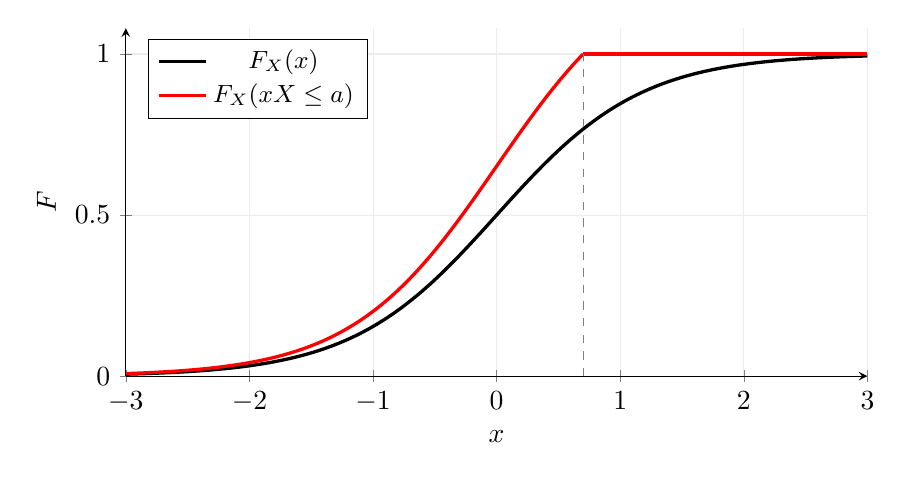
\begin{tikzpicture}
\begin{axis}[width=11cm,height=6cm,axis lines=left,xmin=-3,xmax=3,ymin=0,ymax=1.08,xlabel={$x$},ylabel={$F$},samples=120,legend pos=north west,legend style={font=\small},grid=major,grid style={gray!15}]
\addplot[black,very thick,domain=-3:3] {1/(1+exp(-1.702*x))};
\addlegendentry{$F_X(x)$}
\addplot[red,very thick,domain=-3:0.7] {(1/(1+exp(-1.702*x)))/(1/(1+exp(-1.702*0.7)))};
\addlegendentry{$F_X(x\given X\le a)$}
\addplot[red,very thick,domain=0.7:3,forget plot] {1};
\draw[dashed,gray] (axis cs:0.7,0) -- (axis cs:0.7,1);
\node[below] at (axis cs:0.7,0) {$a$};
\end{axis}
\end{tikzpicture}
\end{center}
(در شکل، $X$ گاوسی استاندارد و $a=0.7$ است.)

\section{خاصیت بی‌حافظگی \lr{(memoryless property)}}

پیش‌تر بیان شد که توزیع نمایی $X\sim\lambda e^{-\lambda x}u(x)$ یک توزیع \textbf{بی‌حافظه} است. این توزیع معمولاً برای مدل‌سازی عمر وسایل الکترونیکی (یا برخی موارد مشابه!) به کار می‌رود.

\begin{definition}[بی‌حافظگی]
یک توزیع روی اعداد نامنفی را \textbf{بی‌حافظه} (\lr{memoryless}) گوییم، اگر به ازای هر $a,\Delta\ge0$ داشته باشیم:
\[
\Prob(X\ge a+\Delta\given X\ge a)=\Prob(X\ge\Delta).
\]
\end{definition}

بی‌حافظه بودن توزیع نمایی به لحاظ ریاضیاتی به صورت زیر اثبات می‌شود (فرض کنید $X\sim\mathrm{Exp}(\lambda)$):
\[
\begin{aligned}
\Prob(X>a+\Delta\given X>a)&=\frac{\Prob(X>a+\Delta)}{\Prob(X>a)}=\frac{1-F(a+\Delta)}{1-F(a)}\\
&=\frac{1-\big(1-e^{-\lambda(a+\Delta)}\big)}{1-\big(1-e^{-\lambda a}\big)}=\frac{e^{-\lambda(a+\Delta)}}{e^{-\lambda a}}=e^{-\lambda\Delta}=\Prob(X>\Delta).
\end{aligned}
\]

\textbf{تعبیر هندسی:} چگالی شرطی $f_X(x\given X>a)$ از بریدن چگالی در $x=a$ و بزرگ‌نمایی (\lr{rescaling}) بخش باقیمانده با ضریب $1/\Prob(X>a)=e^{\lambda a}$ به دست می‌آید. برای توزیع نمایی، نتیجه دقیقاً همان منحنی اولیه است که به اندازه $a$ به راست منتقل شده است:
\[
f_X(x\given X>a)=\frac{\lambda e^{-\lambda x}}{e^{-\lambda a}}=\lambda e^{-\lambda(x-a)},\qquad x>a .
\]

\begin{center}
\begin{tikzpicture}
\begin{axis}[width=10cm,height=5.5cm,axis lines=left,xmin=0,xmax=3,ymin=0,ymax=1.1,xtick={0,1},xticklabels={$0$,$a$},ytick=\empty,samples=100]
\addplot[fill=blue!15,draw=blue!70!black,very thick,domain=0:3] {exp(-x)} \closedcycle;
\addplot[fill=purple!15,draw=purple,very thick,domain=1:3] {exp(-(x-1))} \closedcycle;
\draw[-{Stealth},gray,very thick] (axis cs:1.2,0.301) -- (axis cs:1.2,0.789);
\draw[-{Stealth},gray,very thick] (axis cs:1.7,0.183) -- (axis cs:1.7,0.467);
\draw[-{Stealth},gray,very thick] (axis cs:2.3,0.100) -- (axis cs:2.3,0.243);
\draw[-{Stealth},gray,very thick] (axis cs:2.8,0.061) -- (axis cs:2.8,0.135);
\end{axis}
\end{tikzpicture}
\end{center}

\begin{note}
\notetitle می‌توان نشان داد توزیع نمایی \emph{تنها} توزیع پیوسته بی‌حافظه است (و توزیع هندسی تنها توزیع گسسته بی‌حافظه روی اعداد طبیعی). دلیل: اگر $G(x)=\Prob(X>x)$ آنگاه بی‌حافظگی یعنی $G(a+\Delta)=G(a)G(\Delta)$، و تنها جواب‌های یکنوای این معادله تابعی به صورت $G(x)=e^{-\lambda x}$ هستند.
\end{note}

\section{مدل‌های آماری مخلوط \lr{(Statistical Mixture Models)}}

یک خانواده از توزیع‌های آماری (مثلاً \textbf{خانواده توزیع‌های گاوسی}) را در نظر بگیرید:
\begin{itemize}
\item فرض کنید که برای مشخص کردن هر عضو از خانواده، مجموعه پارامترهای آزاد $\theta\in\Theta$ نیاز باشد.
\item برای مثال، مشخص کردن هر عضو خانواده گاوسی به صورت یکتا از طریق مشخص کردن مقدار میانگین ($\mu$) و واریانس ($\sigma^2$) آن امکان‌پذیر است. پس داریم:
\[
\theta=(\mu,\sigma),\qquad\Theta=\R\times\R_{\ge0}.
\]
\end{itemize}
در این صورت، تابع چگالی احتمال $f_X(x\given\theta)$ نشان‌دهنده یک عضو از خانواده با پارامترهای $\theta$ است.

فرض کنید که متغیر تصادفی $X$، دارای توزیع احتمال متناظر با یکی از $n$ عضو خانواده با پارامترهای $\theta_1,\theta_2,\ldots,\theta_n$ باشد. اما \textbf{این واقعیت که از کدامیک پیروی کند} خود یک متغیر تصادفی گسسته با احتمال‌های $p_1,p_2,\ldots,p_n$ را تشکیل دهد. در این صورت، با توجه به \textbf{قانون احتمال کل} داریم:
\[
\boxed{\ f_X(x)=\sum_{i=1}^{n}p_if_X(x\given\theta_i)\ }
\]
به چنین توزیع‌هایی اصطلاحاً توزیع‌های آماری مخلوط با $n$ خوشه (یا \lr{mixture component}) اطلاق می‌گردد. مثال معروف آن \textbf{مدل مخلوط گاوسی} \lr{(Gaussian Mixture Model --- GMM)} است که در یادگیری ماشین برای خوشه‌بندی داده‌ها کاربرد فراوان دارد. (مسئله دماسنج نامطمئن جلسه قبل نیز یک مدل مخلوط با دو مؤلفه بود.)

\begin{center}
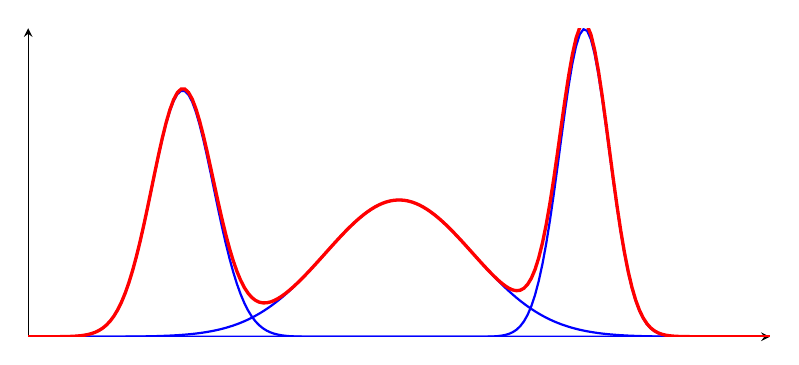
\begin{tikzpicture}
\begin{axis}[width=11cm,height=5.5cm,axis lines=left,xmin=-4,xmax=8,ymin=0,ymax=0.3,xtick=\empty,ytick=\empty,samples=200,domain=-4:8]
\addplot[blue,thick] {0.3*exp(-(x+1.5)^2/(2*0.5^2))/(sqrt(2*pi)*0.5)};
\addplot[blue,thick] {0.4*exp(-(x-2)^2/(2*1.2^2))/(sqrt(2*pi)*1.2)};
\addplot[blue,thick] {0.3*exp(-(x-5)^2/(2*0.4^2))/(sqrt(2*pi)*0.4)};
\addplot[red,very thick] {0.3*exp(-(x+1.5)^2/(2*0.5^2))/(sqrt(2*pi)*0.5)+0.4*exp(-(x-2)^2/(2*1.2^2))/(sqrt(2*pi)*1.2)+0.3*exp(-(x-5)^2/(2*0.4^2))/(sqrt(2*pi)*0.4)};
\end{axis}
\end{tikzpicture}\\
{\small یک \lr{GMM} با سه مؤلفه: منحنی قرمز = مجموع وزن‌دار سه منحنی آبی (وزن‌ها $0.3,0.4,0.3$).}
\end{center}

\begin{note}
\notetitle \textbf{نمونه‌برداری از مدل مخلوط:} ابتدا با احتمال‌های $p_1,\ldots,p_n$ یکی از مؤلفه‌ها (مثلاً $i$) را انتخاب کنید، سپس یک نمونه از $f_X(\cdot\given\theta_i)$ بگیرید. این دقیقاً همان «قانون احتمال کل» به زبان الگوریتم است.
\end{note}

\section{توصیف یک متغیر تصادفی}

فرض کنید که قصد دارید یک متغیر تصادفی را به صورت \textcolor{red!70!black}{ناقص} ولی \textcolor{blue!60!black}{به شکلی ساده} توصیف کنید. مثلاً، کسی که اهل شهر شما نیست در مورد دمای هوا در محل زندگیتان از شما سؤالی می‌پرسد:
\begin{itemize}
\item دمای هوای شهر به شکل یک متغیر تصادفی مانند $T$ مدل‌سازی شده که دارای فضای احتمال و تابع چگالی احتمال $f_T(T)$ است (برای مقادیر $T$ بین صفر کلوین تا بی‌نهایت).
\item ممکن است شما اطلاع دقیقی از تابع توزیع احتمال $T$ داشته باشید. در این صورت تمام چیزی که در مورد دمای هوای شهر می‌توان داشت را دارید.
\end{itemize}
اما جواب آن شخص را چگونه می‌دهید؟ آیا کل تابع چگالی احتمال (شامل بی‌نهایت عدد) را به وی منتقل می‌کنید؟ آیا انتقال این حجم از اطلاعات در مقابل یک پرسش ساده، کاری منطقی به نظر می‌رسد؟ احتمالاً جواب می‌دهید: «معمولاً حدود ۲۵ درجه است، گاهی تا ۳۵ هم می‌رسد».

\subsection{آماره یا \lr{Statistic}}
\begin{itemize}
\item علم آمار و احتمال، در این مواقع ابزارهایی تحت عنوان «\textbf{آماره}» یا «\lr{\textbf{Statistic}}» را در اختیار ما قرار می‌دهد.
\item هر آماره، یک تک عدد و یا مجموعه‌ای نسبتاً کوچکی از اعداد است که اطلاعاتی کلی در مورد یک متغیر تصادفی در اختیار قرار می‌دهد.
\item اطلاعات آماره در مورد یک متغیر تصادفی ناقص است، ولی در عوض انتقال و فهم آن بسیار سریع و راحت می‌نماید.
\end{itemize}

\section{میانگین \lr{(Expected Value)}}

\subsection{مفهوم}
\begin{itemize}
\item معروف‌ترین و پرکاربردترین آماره در تحلیل آماری و تصادفی وقایع، \textbf{میانگین} یا \lr{\textbf{Expected Value}} یک متغیر تصادفی مانند $X$ است.
\item میانگین $X$ را به صورت $\E(X)$ نشان می‌دهیم (به آن \lr{Expectation of $X$} و یا \lr{Mean of $X$} نیز اطلاق می‌گردد).
\item میانگین یک متغیر تصادفی، \textcolor{red!70!black}{\textbf{ماهیت تصادفی نداشته}} و یک مقدار \textcolor{blue!60!black}{\textbf{یقینی}} (\lr{deterministic}) دارد.
\item میانگین برای متغیرهای تصادفی مستقل از پیوسته یا گسسته بودن آنان تعریف می‌شود.
\item امکان تعریف میانگین یا \lr{Expected Value} برای برخی متغیرهای تصادفی وجود ندارد.
\end{itemize}

\subsection{فرمول ریاضی}
\begin{definition}[میانگین]
میانگین یک متغیر تصادفی گسسته با تابع \lr{PMF} برابر با $P(X=x)$ مطابق با زیر تعریف می‌شود:
\[
\E(X)=\sum_{x_i\in\mathrm{supp}(X)}x_iP(X=x_i).
\]
میانگین یک متغیر تصادفی پیوسته (یا مخلوط) با تابع \lr{PDF} برابر با $f_X(x)$ به صورت زیر تعریف می‌شود:
\[
\E(X)=\int_{-\infty}^{\infty}xf_X(x)\dd x .
\]
(به شرطی که سری یا انتگرال به‌طور مطلق همگرا باشد، یعنی $\E|X|<\infty$.)
\end{definition}

\begin{note}
\notetitle \textbf{تعبیر فیزیکی:} اگر \lr{PMF/PDF} را توزیع جرم روی یک میله بدانیم، $\E(X)$ \textbf{مرکز جرم} (نقطه تعادل) آن است. \textbf{تعبیر آماری:} طبق قانون اعداد بزرگ (پایین‌تر)، میانگین تعداد زیادی نمونه مستقل از $X$ به $\E(X)$ نزدیک می‌شود. همچنین برای هر تابع $g$ داریم $\E[g(X)]=\sum g(x_i)P(X=x_i)$ یا $\int g(x)f_X(x)\dd x$.
\end{note}

\subsection{میانگین متغیرهای تصادفی گسسته معروف}

\begin{example}[برنولی، تاس و دوجمله‌ای]
\textbf{برنولی} با احتمال موفقیت $p$:
\[
\E(X)=1\times p+0\times(1-p)=p .
\]
\textbf{تاس ۶وجهی متقارن:}
\[
\E(X)=\frac{1+2+\cdots+6}{6}=\frac{21}{6}=3.5 .
\]
\textbf{دوجمله‌ای} $\mathrm{Binomial}(n,p)$: با استفاده از اتحاد $k\binom nk=n\binom{n-1}{k-1}$:
\[
\E(X)=\sum_{k=0}^{n}k\binom nkp^k(1-p)^{n-k}=np\sum_{k=1}^{n}\binom{n-1}{k-1}p^{k-1}(1-p)^{n-k}=np(p+1-p)^{n-1}=np .
\]
(جمله $k=0$ صفر است؛ و مجموع باقیمانده با تغییر اندیس $j=k-1$ طبق قضیه دوجمله‌ای برابر ۱ است.) به‌طور شهودی: $n$ آزمون، هر یک به طور متوسط $p$ موفقیت.
\end{example}

\begin{example}[هندسی و پواسون]
\textbf{هندسی:} با قرارداد اسلاید، $P(X=k)=(1-p)p^{k-1}$ برای $k\ge1$ (در اینجا $p$ احتمال «ادامه دادن» یا شکست در هر مرحله و $1-p$ احتمال توقف است). با مشتق‌گیری از سری هندسی $\sum_{k\ge0}p^k=\frac1{1-p}$:
\[
\E(X)=\sum_{k=1}^{\infty}k(1-p)p^{k-1}=(1-p)\frac{\partial}{\partial p}\big(1+p+p^2+\cdots\big)=(1-p)\frac{1}{(1-p)^2}=\frac{1}{1-p}.
\]
\textbf{دقت کنید:} در قرارداد جلسه ششم ($P_X(k)=(1-p)^{k-1}p$ با $p$ = احتمال موفقیت) همین محاسبه نتیجه می‌دهد $\E(X)=\frac1p$؛ مثلاً به طور متوسط ۶ پرتاب لازم است تا اولین ۶ در تاس بیاید.

\textbf{پواسون} با پارامتر $\lambda$:
\[
\E(X)=\sum_{k=0}^{\infty}ke^{-\lambda}\frac{\lambda^k}{k!}=\lambda e^{-\lambda}\frac{\partial}{\partial\lambda}\Big(\sum_{k=0}^{\infty}\frac{\lambda^k}{k!}\Big)=\lambda e^{-\lambda}\frac{\partial}{\partial\lambda}\big(e^\lambda\big)=\lambda .
\]
(از $k\lambda^k=\lambda\frac{\partial}{\partial\lambda}\lambda^k$ استفاده شد.) پس پارامتر $\lambda$ همان «تعداد متوسط رخدادها» است ــ سازگار با $np=\lambda$ در تقریب پواسون.
\end{example}

\subsection{میانگین متغیرهای تصادفی پیوسته معروف}

\begin{example}[گاوسی و نمایی]
\textbf{گاوسی} $\mathcal N(\mu,\sigma^2)$:
\[
\E(X)=\frac{1}{\sqrt{2\pi}\sigma}\int_{-\infty}^{\infty}xe^{-\frac{(x-\mu)^2}{2\sigma^2}}\dd x=\mu .
\]
اثبات: با $x=\mu+t$ انتگرال برابر $\mu\int f+\frac1{\sqrt{2\pi}\sigma}\int te^{-t^2/2\sigma^2}\dd t=\mu\cdot1+0$، زیرا انتگرال دوم از یک تابع فرد روی بازه متقارن است.

\textbf{نمایی} با پارامتر $\lambda$: با تغییر متغیر $u=\lambda x$ و انتگرال‌گیری جزءبه‌جزء ($\int_0^\infty ue^{-u}\dd u=[-ue^{-u}]_0^\infty+\int_0^\infty e^{-u}\dd u=1$):
\[
\E(X)=\lambda\int_0^\infty xe^{-\lambda x}\dd x=\frac1\lambda\int_0^\infty ue^{-u}\dd u=\frac1\lambda .
\]
پس اگر نرخ خرابی یک قطعه $\lambda=0.2$ در سال باشد، عمر متوسط آن ۵ سال است.
\end{example}

\begin{note}
\notetitle \textbf{تمرکز مقادیر حول میانگین در توزیع گاوسی:} عمده احتمالات در بازه $\mu\pm3\sigma$ تجمع پیدا کرده است:
$34.1\%$ بین $\mu$ و $\mu+\sigma$، $13.6\%$ بین $\mu+\sigma$ و $\mu+2\sigma$، و $2.15\%$ بین $\mu+2\sigma$ و $\mu+3\sigma$ (و به همین ترتیب در سمت چپ). در مجموع: $68.2\%$ در $\mu\pm\sigma$، $95.4\%$ در $\mu\pm2\sigma$ و $99.7\%$ در $\mu\pm3\sigma$.
\end{note}

\begin{center}
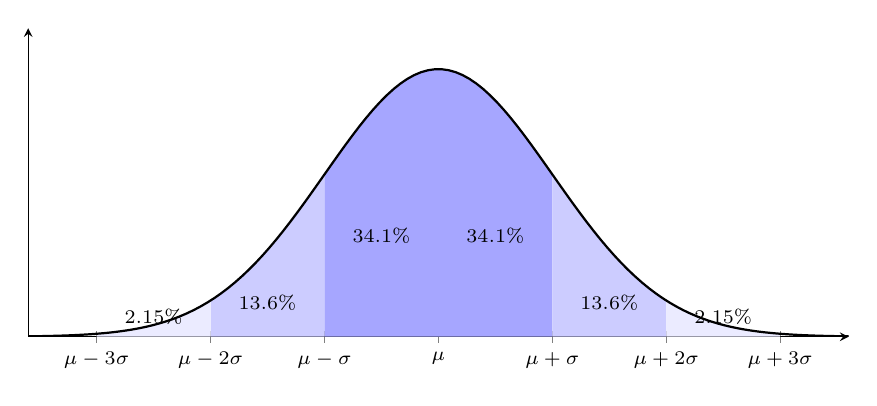
\begin{tikzpicture}
\begin{axis}[width=12cm,height=5.5cm,axis lines=left,xmin=-3.6,xmax=3.6,ymin=0,ymax=0.46,xtick={-3,-2,-1,0,1,2,3},xticklabels={$\mu-3\sigma$,$\mu-2\sigma$,$\mu-\sigma$,$\mu$,$\mu+\sigma$,$\mu+2\sigma$,$\mu+3\sigma$},ytick=\empty,samples=120,tick label style={font=\scriptsize}]
\addplot[fill=blue!35,draw=none,domain=-1:1] {exp(-x^2/2)/sqrt(2*pi)} \closedcycle;
\addplot[fill=blue!20,draw=none,domain=-2:-1] {exp(-x^2/2)/sqrt(2*pi)} \closedcycle;
\addplot[fill=blue!20,draw=none,domain=1:2] {exp(-x^2/2)/sqrt(2*pi)} \closedcycle;
\addplot[fill=blue!8,draw=none,domain=-3:-2] {exp(-x^2/2)/sqrt(2*pi)} \closedcycle;
\addplot[fill=blue!8,draw=none,domain=2:3] {exp(-x^2/2)/sqrt(2*pi)} \closedcycle;
\addplot[black,thick,domain=-3.6:3.6] {exp(-x^2/2)/sqrt(2*pi)};
\node at (axis cs:-0.5,0.15) {\scriptsize $34.1\%$};
\node at (axis cs:0.5,0.15) {\scriptsize $34.1\%$};
\node at (axis cs:-1.5,0.05) {\scriptsize $13.6\%$};
\node at (axis cs:1.5,0.05) {\scriptsize $13.6\%$};
\node at (axis cs:-2.5,0.03) {\scriptsize $2.15\%$};
\node at (axis cs:2.5,0.03) {\scriptsize $2.15\%$};
\end{axis}
\end{tikzpicture}
\end{center}

\begin{example}[یکنواخت و بتا]
\textbf{یکنواخت} در بازه $[a,b]$:
\[
\E(X)=\frac{1}{b-a}\int_a^bx\dd x=\frac{b^2-a^2}{2(b-a)}=\frac{a+b}{2}.
\]
\textbf{بتا} با پارامترهای $\alpha,\beta$: با استفاده از اتحاد تابع بتا $\int_0^1x^{a-1}(1-x)^{b-1}\dd x=\frac{\Gamma(a)\Gamma(b)}{\Gamma(a+b)}$ و $\Gamma(z+1)=z\Gamma(z)$:
\[
\E(X)=\frac{\Gamma(\alpha+\beta)}{\Gamma(\alpha)\Gamma(\beta)}\int_0^1x^{\alpha}(1-x)^{\beta-1}\dd x
=\frac{\Gamma(\alpha+\beta)}{\Gamma(\alpha)\Gamma(\beta)}\cdot\frac{\Gamma(\alpha+1)\Gamma(\beta)}{\Gamma(\alpha+\beta+1)}=\frac{\alpha}{\alpha+\beta}.
\]
\end{example}

\section{خواص میانگین}

\begin{theorem}[برخی خواص میانگین ــ یک متغیر]
فرض کنید $X$ یک متغیر تصادفی گسسته، پیوسته و یا مخلوط باشد و $\E(X)$ وجود داشته باشد. آنگاه:
\begin{enumerate}
\item در صورتی که تابع چگالی احتمال $f_X(x)$ حول نقطه‌ای متقارن باشد، مقدار میانگین نیز برابر با همان نقطه است (مثلاً در مورد متغیرهای تصادفی \textcolor{blue!60!black}{گاوسی} و \textcolor{blue!60!black}{لاپلاس}).
\item لزومی ندارد که خود $\E(X)$ جزو $\mathrm{Support}(X)$ باشد (مثلاً میانگین تاس $3.5$ است که هرگز ظاهر نمی‌شود).
\item همواره داریم: $\ \min(X)\le\E(X)\le\max(X)$.
\end{enumerate}
\end{theorem}
\begin{proof}
(۱) اگر $f_X$ حول $c$ متقارن باشد، $Y=X-c$ چگالی زوج دارد و $\E(Y)=\int yf_Y(y)\dd y=0$ (انتگرال تابع فرد)؛ پس $\E(X)=c$.
(۳) اگر $m\le X\le M$، آنگاه $\E(X)=\int xf\le\int Mf=M$ و به طور مشابه $\ge m$.
\end{proof}

\begin{theorem}[خاصیت خطی \lr{Expectation}]
فرض کنید $X,Y$ متغیرهای گسسته، پیوسته و یا مخلوط باشند و $\E(X)$ و $\E(Y)$ وجود داشته باشند. $X$ و $Y$ \textcolor{red!70!black}{\textbf{لزوماً از یکدیگر مستقل نیستند}}. آنگاه برای اعداد ثابت حقیقی $a,b$:
\[
\E(aX+b)=a\E(X)+b .
\]
به عبارت دیگر، در صورتی که $g$ یک \textbf{تابع خطی} باشد، داریم $\E\big(g(X)\big)=g\big(\E(X)\big)$. همچنین همواره داریم:
\[
\E(X+Y)=\E(X)+\E(Y).
\]
\end{theorem}
\begin{proof}
برای حالت پیوسته: $\E(aX+b)=\int(ax+b)f_X(x)\dd x=a\int xf_X+b\int f_X=a\E(X)+b$.
برای جمع (حالت گسسته): $\E(X+Y)=\sum_{x,y}(x+y)P(x,y)=\sum_xx\sum_yP(x,y)+\sum_yy\sum_xP(x,y)=\sum_xxP_X(x)+\sum_yyP_Y(y)$. دقت کنید که در هیچ جای این اثبات از استقلال استفاده نشد.
\end{proof}

\begin{theorem}[نامساوی \lr{Jensen}]
اگر $g$ تابعی \textbf{محدب} باشد (مثل $x^2$، $e^x$ یا $|x|$)، آنگاه
\[
\E\big(g(X)\big)\ge g\big(\E(X)\big).
\]
(برای تابع مقعر جهت نامساوی برعکس است.)
\end{theorem}
\begin{proof}[ایده اثبات]
تابع محدب بالای خط مماس خود در هر نقطه قرار دارد: با $\mu=\E(X)$، عددی $c$ هست که برای همه $x$: $g(x)\ge g(\mu)+c(x-\mu)$. با میانگین‌گیری از دو طرف (و خاصیت خطی): $\E g(X)\ge g(\mu)+c(\E X-\mu)=g(\mu)$.
\end{proof}

\begin{warning}
\warntitle در حالت کلی $\E(g(X))\neq g(\E(X))$. مثلاً برای تاس: $\E(X^2)=\frac{1+4+9+16+25+36}{6}=\frac{91}{6}\approx15.17$ ولی $(\E X)^2=12.25$. طبق جنسن، اختلاف این دو همیشه نامنفی است (و در جلسه بعد نام «واریانس» می‌گیرد).
\end{warning}

\begin{example}[کاربرد خاصیت خطی ــ تطابق]
$n$ نفر کلاه‌های خود را در یک جعبه می‌اندازند و هر نفر یک کلاه به تصادف برمی‌دارد. میانگین تعداد افرادی که کلاه خودشان را برمی‌دارند چقدر است؟
\begin{solution}
$X_i$ را متغیر برنولی «نفر $i$ کلاه خودش را برداشته» بگیرید؛ $\E(X_i)=\frac1n$. تعداد کل $X=\sum X_i$ است و با خاصیت خطی (با وجود اینکه $X_i$ها مستقل نیستند!):
$\E(X)=\sum_{i=1}^n\frac1n=1$. جالب است که جواب به $n$ بستگی ندارد.
\end{solution}
\end{example}

\section{مفهوم متغیرهای تصادفی \lr{i.i.d.} و قانون اعداد بزرگ \lr{(Law of Large Numbers)}}

فرض کنید که $X_1,X_2,\ldots,X_n$ متغیرهای تصادفی \lr{i.i.d.} از یک توزیع با میانگین $\mu$ باشند. متغیر تصادفی $\bar X_n$ را به صورت زیر تعریف می‌کنیم:
\[
\bar X_n\triangleq\frac{X_1+X_2+\cdots+X_n}{n}.
\]
(دقت کنید که $\bar X_n$ خودش یک متغیر تصادفی است؛ طبق خاصیت خطی $\E(\bar X_n)=\mu$.) آنگاه قانون اعداد بزرگ به دو شکل زیر برقرار است:

\begin{theorem}[قانون اعداد بزرگ]
\textbf{شکل ضعیف:} $\bar X_n\xrightarrow{P}\mu$ وقتی $n\to\infty$؛ یعنی برای هر عدد مثبت $\varepsilon$:
\[
\lim_{n\to\infty}\Pr\big(|\bar X_n-\mu|>\varepsilon\big)=0 .
\]
\textbf{شکل قوی:} $\bar X_n\xrightarrow{\text{a.s.}}\mu$ وقتی $n\to\infty$؛ یعنی
\[
\Pr\Big(\lim_{n\to\infty}\bar X_n=\mu\Big)=1 .
\]
\end{theorem}

\begin{note}
\notetitle شکل ضعیف می‌گوید برای هر $n$ بزرگ، احتمال اینکه میانگین نمونه‌ای از $\mu$ دور باشد کوچک است. شکل قوی بیشتر می‌گوید: تقریباً هر دنباله از نمونه‌ها (به جز مجموعه‌ای با احتمال صفر) در نهایت به $\mu$ همگرا می‌شود. شکل قوی، شکل ضعیف را نتیجه می‌دهد. این قانون توجیه ریاضی تعبیر فرکانسی احتمال است: اگر $X_i=\ind(A\text{ در آزمایش }i)$ باشد، $\bar X_n$ همان فرکانس نسبی است و به $\Prob(A)$ میل می‌کند. (پدیده تمرکز در جلسه سوم نمونه‌ای از همین قانون بود.)
\end{note}

\section{توزیع‌های بدون میانگین}

\begin{definition}[توزیع کوشی \lr{(Cauchy distribution)}]
توزیع کوشی با محلیت (\lr{location}) $x_0$ و مقیاس $\gamma>0$ را با چگالی احتمال زیر تعریف می‌کنیم:
\[
f_X(x)=\frac{1}{\gamma\pi\Big[1+\big(\frac{x-x_0}{\gamma}\big)^2\Big]}.
\]
\end{definition}

\begin{center}
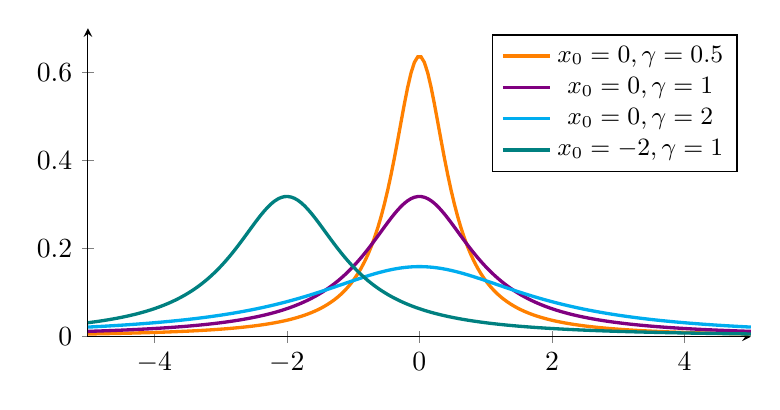
\begin{tikzpicture}
\begin{axis}[width=10cm,height=5.5cm,axis lines=left,xmin=-5,xmax=5,ymin=0,ymax=0.7,samples=200,domain=-5:5,legend style={font=\small}]
\addplot[orange,very thick] {1/(0.5*pi*(1+(x/0.5)^2))}; \addlegendentry{$x_0=0,\gamma=0.5$}
\addplot[violet,very thick] {1/(pi*(1+x^2))}; \addlegendentry{$x_0=0,\gamma=1$}
\addplot[cyan,very thick] {1/(2*pi*(1+(x/2)^2))}; \addlegendentry{$x_0=0,\gamma=2$}
\addplot[teal,very thick] {1/(pi*(1+(x+2)^2))}; \addlegendentry{$x_0=-2,\gamma=1$}
\end{axis}
\end{tikzpicture}
\end{center}

می‌توانید به راحتی ببینید که یک متغیر تصادفی مانند $X$ با توزیع کوشی میانگین ندارد. یعنی $\E(X)$ وجود نداشته و قابل تعریف نیست:
\[
\int_{-\infty}^{\infty}|x|\frac{1}{\pi(1+x^2)}\dd x=\frac{2}{\pi}\int_0^\infty\frac{x}{1+x^2}\dd x=\frac1\pi\Big[\ln(1+x^2)\Big]_0^\infty=\infty .
\]
(دقت کنید که با وجود تقارن چگالی حول صفر، نمی‌توان گفت میانگین صفر است؛ زیرا $\int_0^\infty$ و $\int_{-\infty}^0$ هر دو بی‌نهایت‌اند و $\infty-\infty$ تعریف نشده است. خاصیت تقارن فقط وقتی کار می‌کند که میانگین وجود داشته باشد.)

\begin{note}
\notetitle دقت کنید که این امر در تناقض با هیچ اصلی در آمار و احتمال نیست. تنها لازمه تعریف یک متغیر تصادفی، فضای احتمال $(\Omega,\F,P)$ است که با تعریف یک \lr{CDF} خود به خود صورت می‌پذیرد. \textcolor{red!70!black}{وجود داشتن میانگین شرط تعریف یک متغیر تصادفی نیست.} همچنین قانون اعداد بزرگ برای کوشی برقرار نیست (فرض آن، یعنی وجود $\mu$، برقرار نیست).
\end{note}

دلیل اصلی عدم وجود میانگین برای توزیع کوشی، دم (\lr{tail}) خیلی قوی آن است:
\begin{center}
\renewcommand{\arraystretch}{1.4}
\begin{tabular}{c|c|c|c|c}
توزیع & یکنواخت & گاوسی & نمایی & کوشی\\\hline
رفتار دُم چگالی & $\propto0$ & $\propto e^{-x^2}$ & $\propto e^{-x}$ & $\propto x^{-2}$
\end{tabular}
\end{center}
برای وجود میانگین باید $xf(x)$ انتگرال‌پذیر باشد. با دم $x^{-2}$، $xf(x)\sim\frac1x$ که انتگرالش (لگاریتم) واگراست.

\section{یک مثال تمرینی: سکه تصادفی با احتمال نامعلوم}

\begin{example}[استنتاج بیزی درباره احتمال شیر]
فرض کنید یک سکه تصادفی با احتمال آمدن شیر $p$ در دست داریم. در مورد $p$ هیچ اطلاعی در دست نیست، و تمام اعداد حقیقی بازه $[0,1]$ برای آن شانس برابر دارند. این سکه را $n$ بار به صورت تصادفی پرتاب می‌کنیم و مشاهده می‌شود که $k$ بار شیر ظاهر شده است. در صورت دانسته بودن نتیجه این آزمایش، توزیع احتمال برای «احتمال شیر آمدن سکه $p$» چقدر است؟
\begin{solution}
«هیچ اطلاعی نداریم» یعنی توزیع پیشین $p$ یکنواخت است:
\[
f_{\bm p}(p)=\begin{cases}1 & 0\le p\le1\\ 0 & \text{o.w.}\end{cases}
\]
به شرط $p$، تعداد شیرها دوجمله‌ای است: $P(\text{test}\given p)=\binom nkp^k(1-p)^{n-k}$. با قانون بیز (نسخه چگالی):
\[
f_{\bm p}(p\given\text{test})=\frac{P(\text{test}\given p)f_{\bm p}(p)}{P(\text{test})}=\frac{1}{P(\text{test})}\binom nkp^k(1-p)^{n-k},\qquad0\le p\le1 .
\]
مخرج با قانون احتمال کل (نسخه پیوسته) به دست می‌آید:
\[
P(\text{test})=\int_{\bm p}P(\text{test}\given p)f_{\bm p}(p)\dd p=\int_0^1\binom nkq^k(1-q)^{n-k}\dd q=\binom nk\frac{k!\,(n-k)!}{(n+1)!}=\frac{1}{n+1}.
\]
(از اتحاد تابع بتا با $\Gamma(m+1)=m!$ استفاده شد. جالب است: پیش از آزمایش، همه مقادیر $k=0,\ldots,n$ هم‌احتمال‌اند!) پس
\[
f_{\bm p}(p\given\text{test})=(n+1)\binom nkp^k(1-p)^{n-k}=\frac{\Gamma(n+2)}{\Gamma(k+1)\Gamma(n-k+1)}p^{k}(1-p)^{n-k},
\]
که دقیقاً چگالی توزیع بتا است. \textbf{جواب نهایی}:
\[
\boxed{\ \bm p\given\text{test}\ \sim\ \mathrm{Beta}(k+1\ ,\ n-k+1)\ }
\]
\end{solution}
\end{example}

\begin{note}
\notetitle طبق فرمول میانگین بتا، $\E(\bm p\given\text{test})=\frac{k+1}{n+2}$ (معروف به «قاعده توالی لاپلاس»). مثلاً اگر در ۱۰ پرتاب ۷ شیر بیاید، تخمین ما $\frac{8}{12}\approx0.67$ است (نه دقیقاً $0.7$). با افزایش $n$، توزیع پسین حول $\frac kn$ باریک‌تر می‌شود. این مثال نشان می‌دهد چرا توزیع بتا برای مدل‌سازی «خود احتمال» مناسب است.
\end{note}

\begin{center}
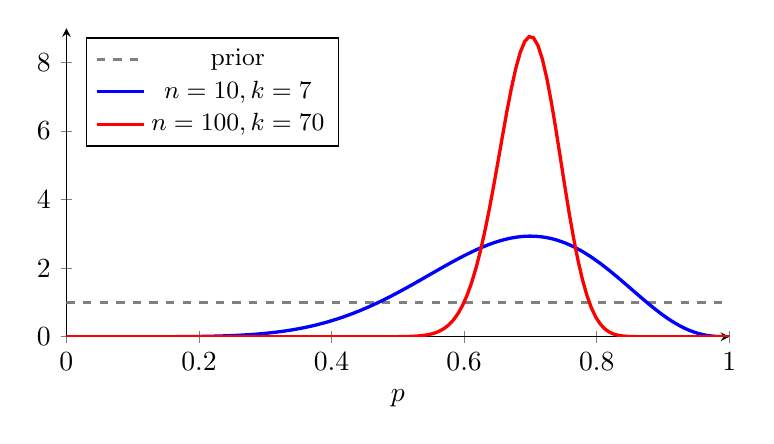
\begin{tikzpicture}
\begin{axis}[width=10cm,height=5.5cm,axis lines=left,xmin=0,xmax=1,ymin=0,ymax=9,xlabel={$p$},samples=150,domain=0:1,legend style={font=\small},legend pos=north west]
\addplot[gray,thick,dashed] {1}; \addlegendentry{\lr{prior}}
\addplot[blue,very thick] {11*120*x^7*(1-x)^3}; \addlegendentry{$n=10,k=7$}
\addplot[red,very thick] {2.9666e27*x^70*(1-x)^30}; \addlegendentry{$n=100,k=70$}
\end{axis}
\end{tikzpicture}
\end{center}

\section{تمرین‌های تکمیلی}

\begin{exercise}
$X$ دارای چگالی $f(x)=2x$ روی $[0,1]$ است. $\E(X)$ و $\E(X^2)$ را بیابید و نامساوی جنسن را برای $g(x)=x^2$ بررسی کنید.
\end{exercise}
\begin{solution}
$\E(X)=\int_0^12x^2\dd x=\frac23$ و $\E(X^2)=\int_0^12x^3\dd x=\frac12$. داریم $\frac12\ge\big(\frac23\big)^2=\frac49\approx0.444$ که با جنسن سازگار است.
\end{solution}

\begin{exercise}
در یک بازی، تاسی پرتاب می‌کنید و اگر عدد $k$ بیاید $k^2$ هزار تومان می‌برید. اگر هزینه ورود ۱۵ هزار تومان باشد، آیا بازی به نفع شماست؟
\end{exercise}
\begin{solution}
سود متوسط $\E(X^2)-15=\frac{91}{6}-15=\frac16\approx0.17$ هزار تومان؛ پس بازی به‌طور متوسط اندکی به نفع بازیکن است. (دقت کنید $(\E X)^2=12.25<15$؛ استفاده نادرست از $g(\E X)$ نتیجه را برعکس می‌کرد.)
\end{solution}

\begin{exercise}
یک کلکسیونر می‌خواهد همه $N$ نوع کارت را جمع کند؛ هر بسته یک کارت تصادفی (یکنواخت) دارد. میانگین تعداد بسته‌های لازم را بیابید (مسئله جمع‌آوری کوپن).
\end{exercise}
\begin{solution}
وقتی $i$ نوع جمع شده است، هر بسته جدید با احتمال $\frac{N-i}{N}$ نوع تازه می‌دهد؛ پس تعداد بسته‌های لازم برای نوع بعدی هندسی با میانگین $\frac{N}{N-i}$ است. با خاصیت خطی:
$\E(T)=\sum_{i=0}^{N-1}\frac{N}{N-i}=N\big(1+\frac12+\cdots+\frac1N\big)\approx N\ln N$. برای $N=50$: حدود $225$ بسته.
\end{solution}
